\documentclass[8pt,twocolumn]{article}
\usepackage[8pt]{extsizes}
\usepackage[utf8]{inputenc}
\usepackage{graphicx}
\usepackage{multicol}
\usepackage{hyperref}
\usepackage{enumerate}
\usepackage{float}
\usepackage[top=2.25cm,bottom=2.25cm,left=2cm,right=2cm,nohead,nofoot]{geometry}
\renewcommand{\thesection}{\largesize{\Roman{section}.}}
\renewcommand{\thesubsection}{\normalsize{\Alph{subsection}.}}
\graphicspath{{Lab3TIIT/}}
\DeclareGraphicsExtensions{.pdf,.png,.jpg}



\title{\huge\textbf{ Ontological Approach to the automated design
of complex systems using aircraft as
an example}
}

\author {
\begin{tabular}[t]{c@{\extracolsep{1em}}c}
  Anastasiya Malochkina & Nikolai Borgest \\
    \textit{Samara University} & \textit{Samara University, ICCS RAS}  \\
    Samara, Russia & Samara, Russia \\
    \href{mailto:malochkina.anastasia@gmail.com}{malochkina.anastasia@gmail.com} & \href{mailto:borgest@yandex.ru}{borgest@yandex.ru} \\
\end{tabular}         
        }

\date{}

\begin{document}
\maketitle
\textbf{\textit{Abstract}—This article discusses the process of complex
systems automation. The analysis of some existing approaches based on the use of ontologies was made: a RobotDesigner created at Samara University and the Design
Cockpit 43®, a compiler using design languages, created
at University of Stuttgart. For the Robot-Designer, the
formalization of knowledge, design procedures and operations in the chosen field of knowledge is considered, along
with semantic and mathematical models. A special place
in the creation of a robot designer takes an interface that
provides the designer with information for making a final
decision and, if necessary, “explains” the need to choose
a specific solution. For the Design Cockpit 43® there is a
description of design languages is given: vocabulary, rules,
grammar, structure of information within the language.
Graph-based design languages are presented as a method
to encode and automate the complete design process and
the final optimization of the product or complex system.
The description and methods of ontology implementation
are given. The task is to consider already existing methods
of automation of aircraft design. It affects the formalization
of the design process as such and, accordingly, the stages
at which it is most advisable to automate human activities.
Examples show how to put it into practice in the modern
production of this kind of automation. The results achieved
and possible future development prospects are indicated.
The relevance of the article is justified by the growing
interest in the automation of design and production since
it reduces the time for design and reduces the number of
errors caused by human factors in both the early and the
later stages of product development. Also, automation of
design gives more spare time to designers which can be
used for the solution of more complex problems. This leads
to rise in the quality of an end product.

\textit{Abstract}—ontology approach, Design Cockpit, RobotDesigner, automated design.}

\begin{center}
\section{Introduction}
Design is a complex decision making process in conditions
of an indeterminateness. At present, when designing complex
systems, it is necessary to understand that they represent a
network of objects interacting in various fields of knowledge
(for example, in mechanics, electrics, etc.). A successful understanding of their interaction is determined by an all-around
theoretical understanding of this system and an understanding
of the process of its design. Traditional approaches today are
associated with the active participation of people at all stages
of design, despite the fact that there are already many standard
solutions that need to be automated. The software is used as
a tool, and not as an intellectual assistant to the designer, as
for the most part, there is no accumulated knowledge base in a
particular subject area. The difference between the considered
approaches in a much deeper formalization of processes based
on ontologies of subject areas. Automation should be implemented to routine, repetitive processes. Finding and correcting
errors made during these processes can significantly increase
the design time. Thus, the automation of the entire product life
cycle helps engineers to solve more important and complex
tasks, which will certainly lead to a reduction in design time and
improve product quality. In the future, success in the industrial
sector will be determined by the use of various information
technologies to support the design and production processes,
but now we can face several problems, which are:
\begin{itemize}
  \item Separated data sources, which is caused by a data structure that represents fragmented “islands”, each of which is a certain knowledge of the subject, but which are difficult to combine together.
  \item The inconsistency of the process arises as a result of the fact that not all processes are established. Each company has its own vision of the process. 
  \item Data exchange as a written documents implies that part of the design time is spent not on the design itself, but on reading documents that describe the previous work.
  \item Creating and updating models manually, as in most cases, to research an object, it is necessary to create different models for different purposes.
\end{itemize}    
\end{center}

\begin{center}
\section{DESIGN COCKPIT 43®}    
\end{center}
\subsection{Formalization of the design process}
The overall design sequence is presented in Figure 1. The red arrows show that the transition to the next stage is possible only with the successful completion of the current one, and the yellow arrows show that if it is impossible to find a solution at this stage, you should return to the earlier design stages and make changes to them. It should be noted that the zero stage is expedient only if it is automated.

Due to the antagonistic design principles “form follows function” and “function follows form”, geometry and physics are potentially both at the same time a requirement or result of a design process, depending on the design context. In graphbased design languages the representation of geometry and physics is called abstract, since both geometry and physics (i.e. loads, boundary conditions, materials) are represented \begin{figure}[h]
    \centering
    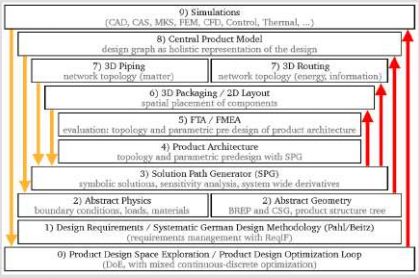
\includegraphics[scale=0.7]{Figure1.png}
    \caption{Figure 1. Design sequence.}
    \label{Fig1:image}
\end{figure}[]
independently of any vendor specific, proprietary data format or tool in the Unified Modeling Language (UML). At the conceptual design stage, geometry is often presented as parameters and fixtures. At stage 3, all necessary calculations are performed. At stage 4, the interaction of components is detected, after which, at stage 5, an analysis of failures is performed by methods such as FTA and FMEA. Next, the layout of the components is drawn up, and the pipes and cables are wired. Stage 8 is possible using the design languages used in the Design Cockpit 43® software [1].
\subsection{Description of design language}
A design language allows for a holistic description of engineering tasks and is words that form some vocabulary and rules that make up some grammar.

The rules encode model transformations, create instances, and work with separate vocabulary blocks, which, in turn, are encoded in the extended UML instance diagram. The set of all rules is called the production system, which is encoded in the UML action diagram. These three parts form a graphbased design language and must be created manually by one or more people as an advance contribution to the engineering design process. When a production system is executed by a so-called design compiler (for example, Design Cockpit 43®), the design result automatically created and stored in the central model is called a graph, that is, a complete digital model of the system containing all parts, connections and parameters. From this central data model, all other necessary system models are generated automatically. For example, you can generate a CAD model or a wiring model.

Here the design language means that all valid sentences in the grammar (that is, all regular combinations of words) are alid in the design of the system. The term “graph-based” means that a single node in a graph serves as an abstract placeholder for a design knowledge element (i.e. Concepts, values, physical component or their totality), and graph edges express (potentially N-dimensional and interdisciplinary) links between different nodes (i.e. different parts of design knowledge). On the example of a car: “Words are a car, wheels, a door.” Rules: (A) if there is nothing, create a car, (B) if there is a car, create its wheels, (C) if there is a car wheel, attach the door. Then production takes the following form: (A) once, (B) once, (C) four times. The resulting graphic scheme has one auto-mobile with wheels and 4 doors.
\subsection{Aviation approach}
Design languages is applicable in a small scope, e.g. the automation of a specific task in an established design process. Figure 2 shows the automation of parts of the design process of an aircraft cabin, with the generation of fioorplan, 3D-model and wire harness model. Automated design of an aircraft cabin including routing. From left to right: a set of requirements (not shown) drives the generation of the cabin layout, manual intervention is possible, e.g. to move the door to another frame if desired. According to the layout pre-constructed geometry is placed to generate a CAD-model. This then allows to calculate the maximum installation space for cables, the routing space. In this routing space network components, e.g. electronic boxes, are placed as start and end points for the routing algorithm. As last step the Design Cockpit 43’s routing algorithm generate the cables and the electrical wire harness. \begin{figure}[h]
    \centering
    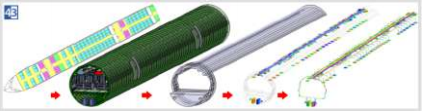
\includegraphics[scale=0.7]{Figure2.png}
    \caption{Figure 2. Automation of parts of the design process.}
    \label{Fig2:image}
\end{figure}
The composition of the cabin harness is directly coupled with the cabin layout. For each seating row there is an overhead panel which includes reading lamps, buttons to call for flight attendees etc. additionally there may be an in-flight entertainment system with screens and audio jacks. These functions are driven by a small electronic box installed on top of the ceiling panel of the seating row. Depending on the chosen electrical architecture these small boxes are in turn connected to bigger management nodes. The number of managed boxes determines the size of those management nodes - a point for optimization, a few big or many small ones. Thus the number and positions of the seats determines directly the position and number of the electronic components which in turn define the harness length and architecture. The automated design process begins with the generation of a cabin layout from a set of requirements, e.g. evacuation times, seat distances, passenger capacity, and so on. The cabin layout can be visualized with an automatically generated fioorplan. Once the layout is fixed the CAD-model of the cabin interior is generated by loading pre-defined 3D-geometry, e.g. seats or overhead bins, at the respective coordinates. Now the routing space can be extracted, this is the maximum possible volume where cables could be placed. Components of the electrical network, e.g. electronic boxes, are placed inside the routing space as start and endpoints for the routing algorithm. In a last step, the Design Cockpit 43’s routing algorithm generates the wire harness of the aircraft cabin. With this automated process in place, quick variation studies in the form of “What happens if...” are possible, e.g. the door is moved by one (fraction of a) frame or the lavatory to passenger ratio is changed [1].

\begin{center}
\section{ROBOT-DESIGNER}
\end{center}
\subsection{Knowledge formalization}
The task of simulating the activities of a project involves not only describing the project operations themselves and the procedures performed, but also translating them into a formal action language. Thus, the initial phase of any pre-project study involves the study of the experience and properties of already created artifacts; This may affect the parameters of the future project.

In the conceptual design of the aircraft, such studies are carried out on the basis of the study of trends, the construction of statistical models. To formalize this process, a database of airplanes, engines, aerodynamic profiles, avionics, etc. is created and updated. Based on the experience, the most demanded and influencing dependencies of the desired parameters that “help” the designer in assessing and making decisions are influenced. All these actions are described, logged and further formalized.

Until recently, difficultly formalized tasks, for example, like the automatic construction of a grid of finite elements on a geometric model, are more subject to the software packages that are being created. 

Having achieved in a number of areas the formalization of knowledge through the identified laws, physical and heuristic patterns, for the further translation of knowledge to a computer, the task of semantic data consistency came to the fore.

An ontology in the form of a thesaurus explicitly provides the information necessary to understand the term in a terminological system, which is the complete semantic environment of each term connected by a semantic network. Small part of this description presented in figure 3.
\begin{figure}[h]
    \centering
    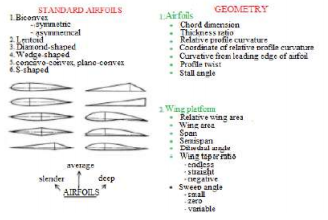
\includegraphics[scale=0.7]{Figure3.png}
    \caption{Figure 3. Example of wing parameters description.}
    \label{Fig3:image}
\end{figure}[]
The ontological approach to the study and research of the domain makes it possible to view the entire set of words, which can be used to describe the topic of interest, while reviewing the semantic environment in which it is interested. The terminology base and methods for its expansion may change both during the creation and use of the thesaurus, therefore, to determine information materials on the domain, the relevance of sources and scenarios for the use of ontology are taken into account.
\subsection{Design Scenario}
Aircraft pre-design is chosen as the Subject Area for the Designer Robot. On the one hand, this is a field of activity that has always required creative solutions, on the other - it is fairly well formalized. The result of the work of the Robot Designer is the model of the aircraft. The preliminary design stage of the aircraft includes the development of a general concept of the designed object, the compilation of models of the object elements, the preparation of a feasibility study, the formation of a design task.

The description of the object includes its design scheme, approximate estimation of mass, overall dimensions and energy consumption.

The Robot-Designer is a computer with peripheral devices, toolkits that include machine description languages, a database management system (DBMS), CAD systems, ontology editors, and a knowledge base, as a combination of thesaurus, database, rules and procedures, with design scenarios. The enlarged block diagram of the Robot-Designer is presented in Figure 4. 

The Robot-Designer can work in the automatic mode or in the mode of the intellectual assistant of the human designer,\begin{figure}[h!]
    \centering
    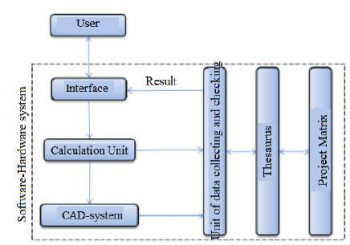
\includegraphics[scale=0.7]{Figure4.png}
    \caption{Figure 4. Structure of Robot-Designer.}
    \label{Fig4:image}
\end{figure}
and the degree of human participation in the design is not constant and depends on the desire of the user. In other words, for each user, in advance or dynamically in the process of work, a communication script is created, including the degree of automation of the design process, the choice of preferred input / output devices, the need to perform certain stage of design. Developed by the Robot-Designer, due to hardware and software limitations, it is not able to independently synthesize fundamentally new versions of the design-power circuit, so the system uses those versions of the design patterns that were previously described in it.

The Robot-Designer allows analyzing a number of variants of the aircraft’s layouts and configurations, either independently or, if necessary, on the basis of a dialogue with the designer, select the option that best meets the specified technical requirements.

Developed Robot-Designer, due to hardware and software limitations, it is not able to independently synthesize fundamentally new versions of the design-power circuit, so the system uses those versions of the design patterns that were previously described in it.

The Robot-Designer allows analyzing a number of variants of the aircraft’s layouts and configurations, either independently or, if necessary, on the basis of a dialogue with the designer, select the option that best meets the specified technical requirements.
\subsection{Geometry model}
In work the method is used, allowing to create geometrical models of the plane in an automatic mode with the help of parametric modeling technology. Any design process as a set of methods of analysis and synthesis includes a set of rules and methods. They can be generalized and implemented by software into some kind of convolution, conventionally called “parametric template”. When using templates, the designer only needs to enter input data. At the output, whole constructions are built according to the knowledge and algorithms for solving problems laid down in the template. Templates enable the once created algorithms to be re-applied to other constructions, while obtaining a new result.

Figures 5 and 6 show the created 3D geometric models of the aircraft, Figure 7 shows the resulting structural-power and volumetric layout of the aircraft. These models can be used as a basis for subsequent engineering analysis in CAE-systems, as well as for physical experiments on a solid-state model obtained on a 3D printer. Figure 5 shows the constructed 3D geometric model of
the aircraft, Figure 6 shows the resulting structural-power and volumetric layout of the aircraft.
\end{document}
